\documentclass[12pt,a4paper]{article}
\usepackage[utf8]{inputenc}
\usepackage[english]{babel}
\usepackage[T1]{fontenc}
\usepackage{amsmath}
\usepackage{amsfonts}
\usepackage{amssymb}
\usepackage{graphicx}
\usepackage{siunitx}
\usepackage{float}
\usepackage[left=2cm,right=2cm,top=2cm,bottom=2cm]{geometry}
\author{Gerald}

\begin{document}
\sisetup{separate-uncertainty = true}
	\setlength{\parindent}{0pt} 
	\begin{center}
		{\LARGE Experiment protocol}\\
		\begin{large}
			for the solid state lab course\\[0.4cm]
			at RWTH Aachen\\
			II. Physikalisches Institut A\\[5.5cm]
			\Large\textbf{\textsl{Superconductivity and SQUID}}\\[5.5cm]
			\normalsize\textit{authored\\by}\\[0.4cm]
			\large{Moritz Berger (355244)\\Gerald Kolter (355005)}\\[2cm]
			\large \textbf{Summer term 2019}
		\end{large}
	\end{center}
	\newpage
	
	\tableofcontents
	\newpage

\section{Impact of the Laser wavelength}
The encapsulated graphene is used to analyze the impact of the Laser wavelength on the Raman spectrum. The $\omega_g$ vs. $\omega_{2D}$ map and $\Gamma_g$ vs. $\Gamma_{2D}$map are shown in figure \ref{fig:Laser_omega} for both Lasers. The distribution of the individual positions are also shown in figure \ref{fig:Laser_omega_hist}.\\
The $\omega_g$ position is not shifted at all. However the $\omega_{2D}$ position shifted from an average position of \SI{2719(3)}{cm^{-1}} for the blue laser to \SI{2683(3)}{cm^{-1}} for the green laser. The reason for this is that only a single electron/hole site participates in the Raman process that leads to the G-line. By changing the Laser frequency only the excitation energy changes. The Raman shift stays the same. The 2D-line requires two lattice sites and the phonon modes connect them. Changing the excitation energy also changes the phonon modes and with that the Raman shift.\\
The higher energy of the blue laser also shifts the average FWHM, as seen in figure \ref{fig:Laser_gamma_hist}. $\Gamma_g$ is larger on average for the blue laser, while $\Gamma_{2D}$ is smaller compared to the green laser. In general the measurement taken with the blue laser seems to be broadly distributed. However this is most likely a consequence of different measurement settings.\\
\\

\begin{figure}
\centering
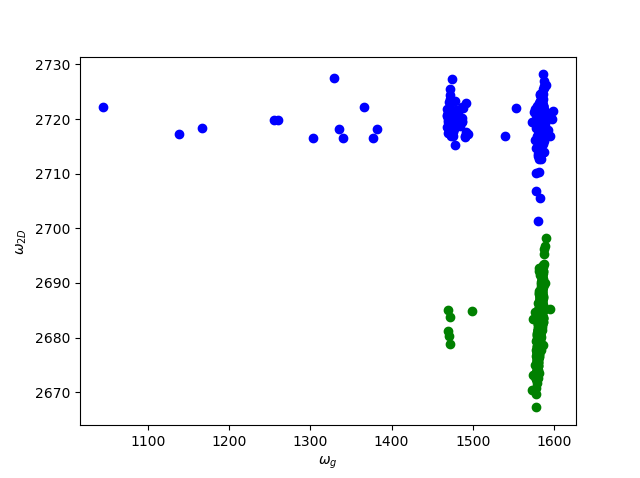
\includegraphics[scale=0.5]{Bilder/Laser/omega.png}
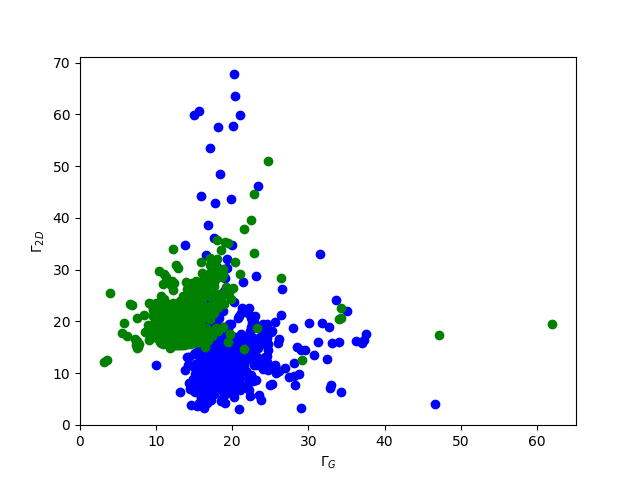
\includegraphics[scale=0.5]{Bilder/Laser/gamma.png}
\caption{line data of the G-line plotted against the 2D-line for both Lasers. Left: $\omega$, right: $\Gamma$. The Data point of the green laser are plotted in green and the blue laser in blue.}
\label{fig:Laser_omega}
\end{figure}

\begin{figure}
\centering
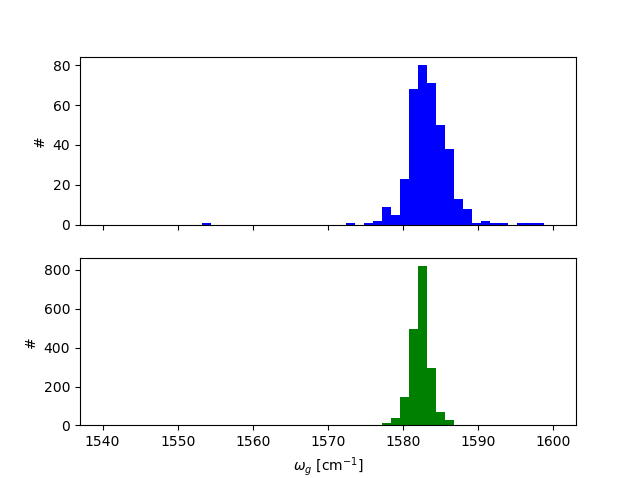
\includegraphics[scale=0.5]{Bilder/Laser/omegag_hist.png}
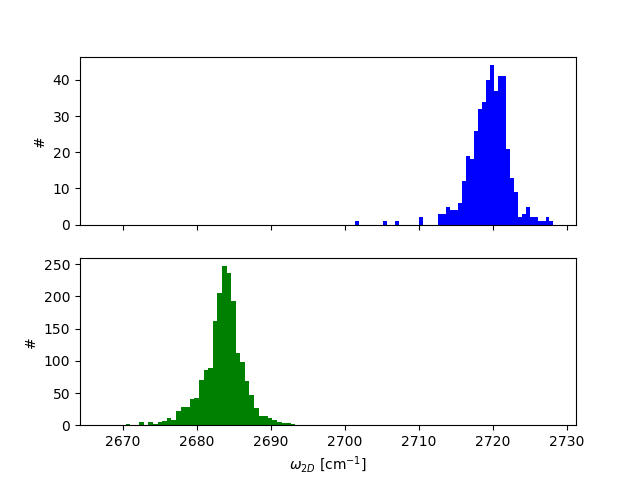
\includegraphics[scale=0.5]{Bilder/Laser/omega2d_hist.png}
\caption{Distribution of the line positions for the blue(top) and green(bottom) Laser. Right: $\omega_{g}$, left: $\omega_{2D}$.}
\label{fig:Laser_omega_hist}
\end{figure}

\begin{figure}
\centering
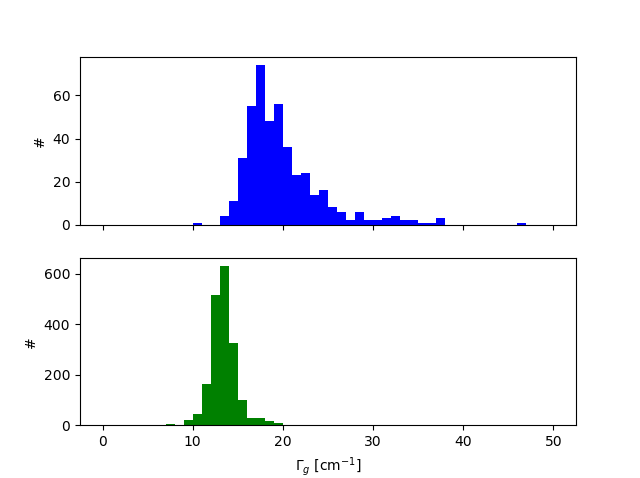
\includegraphics[scale=0.5]{Bilder/Laser/gammag_hist.png}
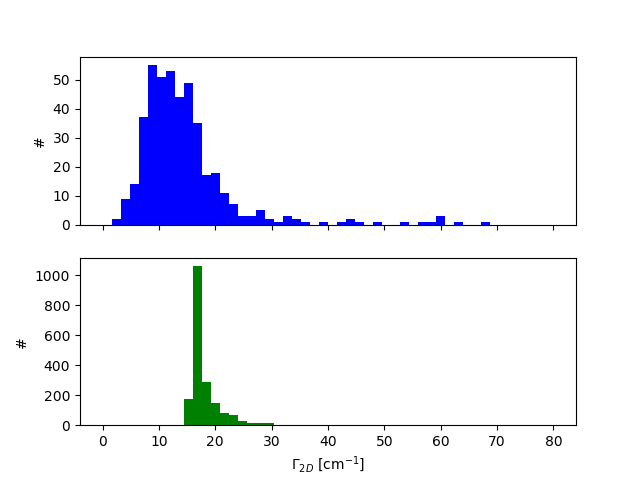
\includegraphics[scale=0.5]{Bilder/Laser/gamma2d_hist.png}
\caption{Distribution of the FWHD for the blue(top) and green(bottom) Laser. Right: $\Gamma_{g}$, left: $\Gamma_{2D}$.}
\label{fig:Laser_gamma_hist}
\end{figure}

\section{polycritalline Cu sample}
This sample is used to analyze the strain of CVD graphene on on a Cu-substrate for different lattice orientations. The Raman-measurement is done with the blue laser.\\ In a first step the $\omega_{g/2D}$ positions for pristine graphene when using this laser are determined and used as reference for the strain calculation. The spectrum of pristine graphene is shown in figure \ref{fig:pristine}. Both lines have a very low intensity, which indicates that there was no graphene at the point where the spectrum was taken. The 2D-line can be analyzed, which results in  $\omega_{2D} = \SI{2721.1(4)}{cm^{-1}}$. However the G-line intensity is too small to be analyzed. Based on the previous chapter we can assume that the G-line does not shift when changing the laser. This means the Raman of this line should be the same as in the spectrum of pristine graphene taken with the green laser, which is shown in figure \ref{fig:pristine_green}. The G-line frequency is $\omega_{G} = \SI{1582.4(3)}{cm^{-1}}$.\\
\\
The polycristalline sample and the measurement points is shown in figure  \ref{fig:poly_sample}. 


\begin{figure}
\centering
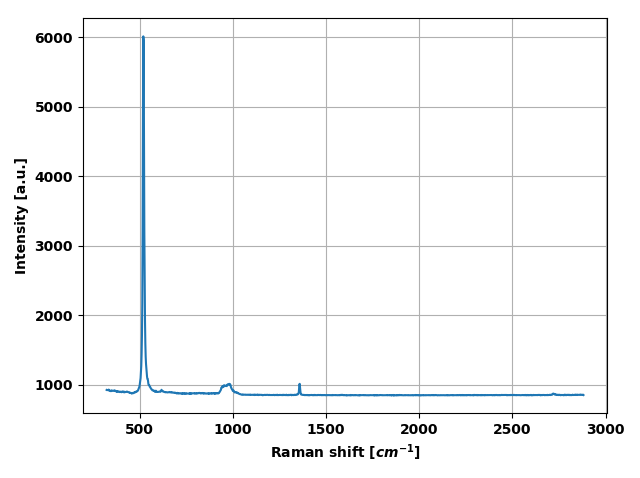
\includegraphics[scale=0.5]{Bilder/part6/prestine_spectrum.png}
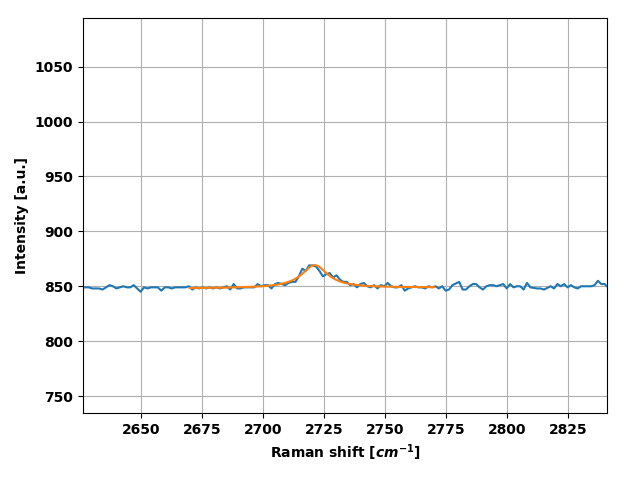
\includegraphics[scale=0.5]{Bilder/part6/prestine_2D.png}
\caption{Spectrum of pristine graphene measured with the blue laser and the same spectrum zoomed into the 2D-line. The G-line is not visible and the 2D-line has a very small intensity. The 2D-line position is $\omega_{2D} = \SI{2721.1(4)}{cm^{-1}}$.}
\label{fig:pristine}
\end{figure}

\begin{figure}
\centering
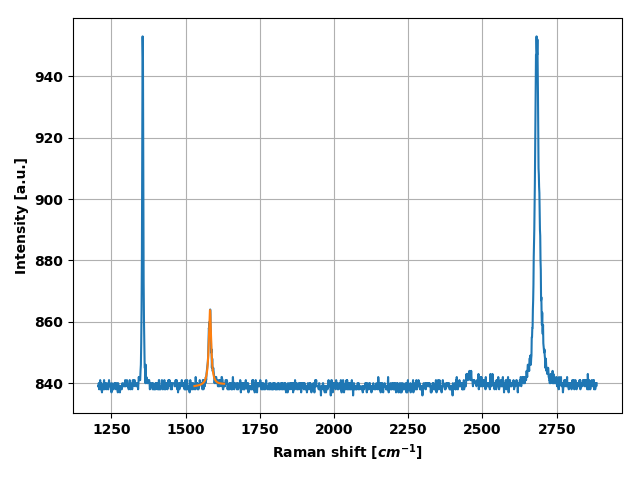
\includegraphics[scale=0.5]{Bilder/part6/prestine_green.png}
\caption{Spectrum of pristine graphene measured with the green laser in order to determine the position of the G-line. The G-line is highlighted and determined with $\omega_{G} = \SI{1582.4(3)}{cm^{-1}}$.}
\label{fig:pristine_green}
\end{figure}

\begin{figure}
\centering
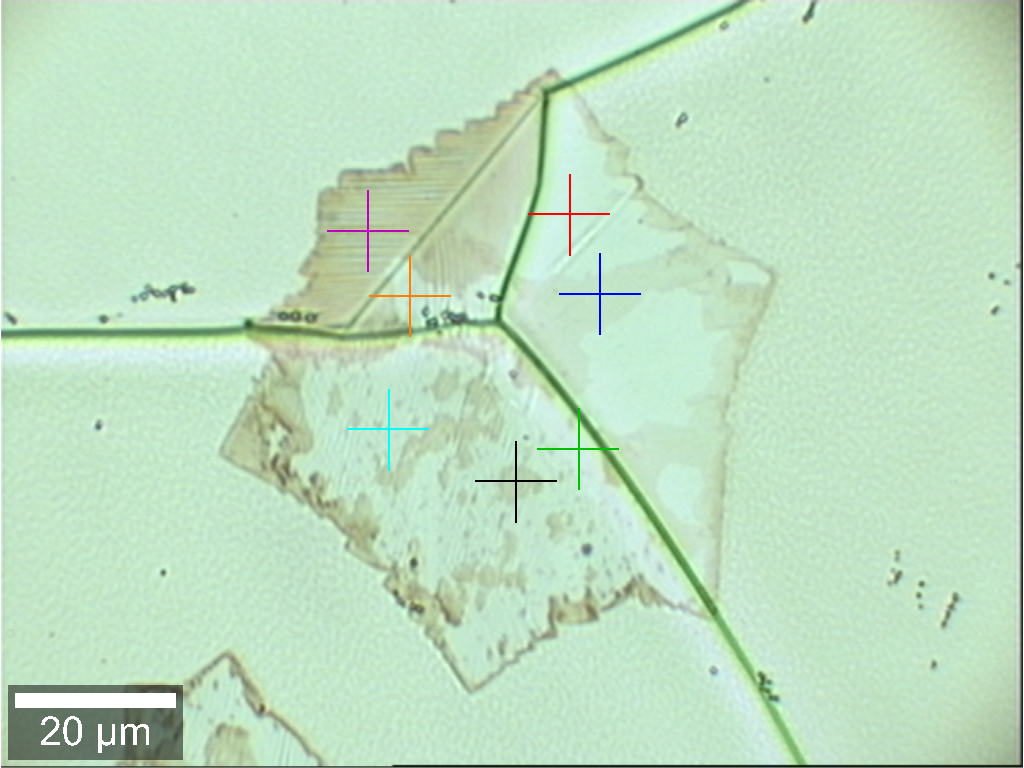
\includegraphics[scale=0.4]{Bilder/part6/4D4RamanFlake.png}
\caption{Polycristalline sample. Measurement points in order of red, blue, green, black, cyan, orange, purple.}
\label{fig:poly_sample}
\end{figure}

\begin{table}[h]
\centering
\begin{tabular}{|c|c|c|c|}
\hline 
Measurement & Miller indices & $\omega _G$ &  $\omega _{2D}$\\ 
point &  &  & \\ 
\hline 
1(red) & (0.14,0.51,0.85) &\SI{1581.4 \pm 0.3}{\per cm} & \SI{2719.4 \pm 0.2}{\per cm}\\ 
\hline 
2(blue) & (0.14,0.51,0.85) & \SI{1583.8 \pm 0.2}{\per cm} & \SI{2701.7 \pm 0.2}{\per cm}\\ 
\hline 
3(green) & (0.33,0.56,0.76) & \SI{1586.4 \pm 0.2}{\per cm} & \SI{2722.8 \pm 0.5}{\per cm}\\ 
\hline 
4(black) & (0.33,0.56,0.76) & \SI{1579.8 \pm 0.2}{\per cm} & \SI{2705.3 \pm 0.4}{\per cm}\\ 
\hline 
5(cyan) & (0.33,0.56,0.76) & \SI{1581.1 \pm 0.3}{\per cm} & \SI{2696.4 \pm 0.5}{\per cm}\\ 
\hline 
6(orange) & (0.03,0.14,0.99) & \SI{1586.4 \pm 0.3}{\per cm} & \SI{2729.0 \pm 0.5}{\per cm}\\ 
\hline 
7(purple) & (0.03,0.14,0.99) & \SI{1583.9 \pm 0.2}{\per cm} & \SI{2702.9 \pm 0.3}{\per cm}\\ 
\hline 
\end{tabular} 
\caption{Results for the positions of G and 2D peak from the polycristalline sample at the measurement points as marked in Fig. \ref{fig:poly_sample}.}
\label{tab:Sandwich_Results}
\end{table}

\section{Appendix}
\begin{figure}
\centering
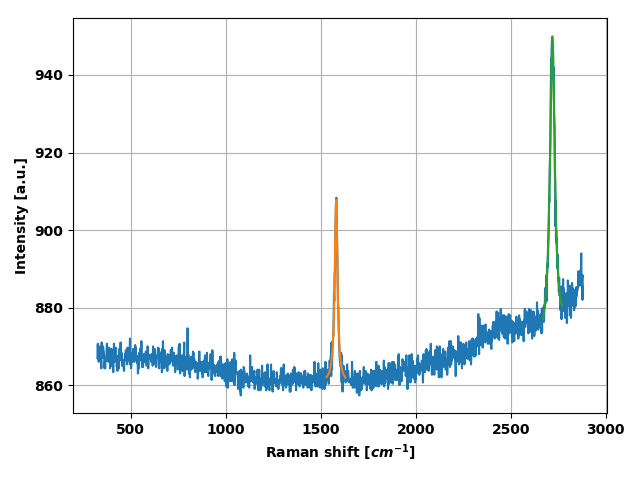
\includegraphics[scale=0.5]{Bilder/part6/1.png}
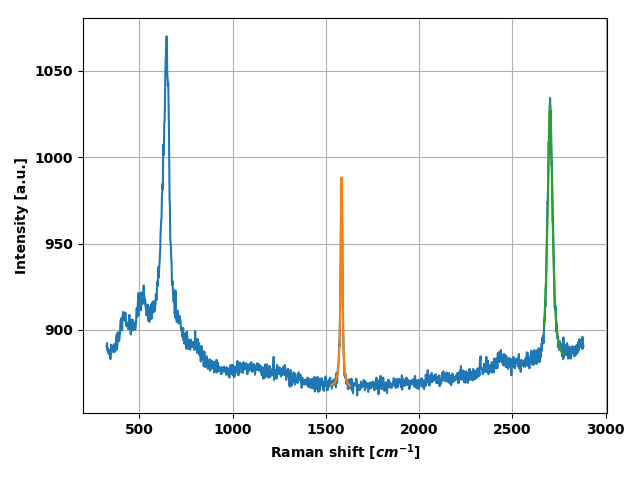
\includegraphics[scale=0.5]{Bilder/part6/2.png}
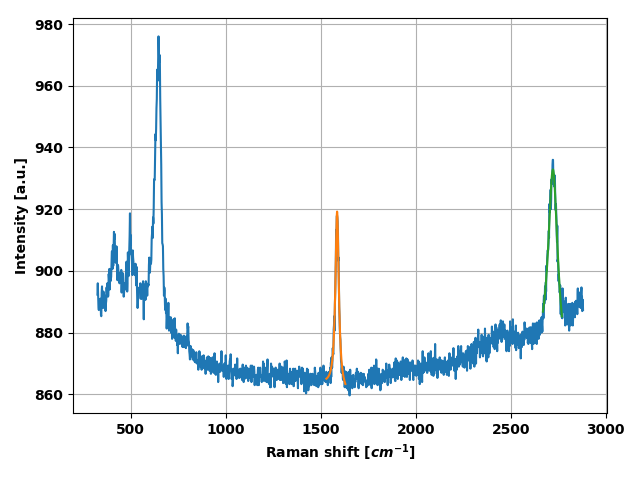
\includegraphics[scale=0.5]{Bilder/part6/3.png}
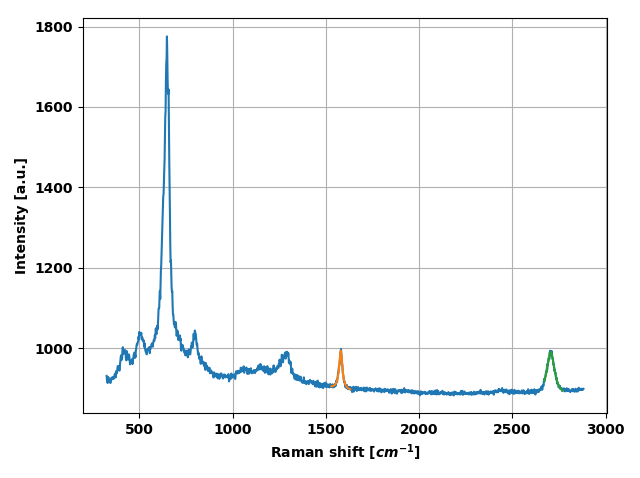
\includegraphics[scale=0.5]{Bilder/part6/4.png}
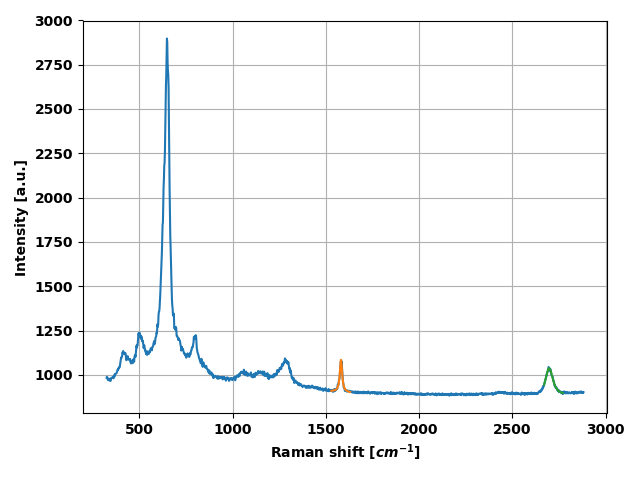
\includegraphics[scale=0.5]{Bilder/part6/5.png}
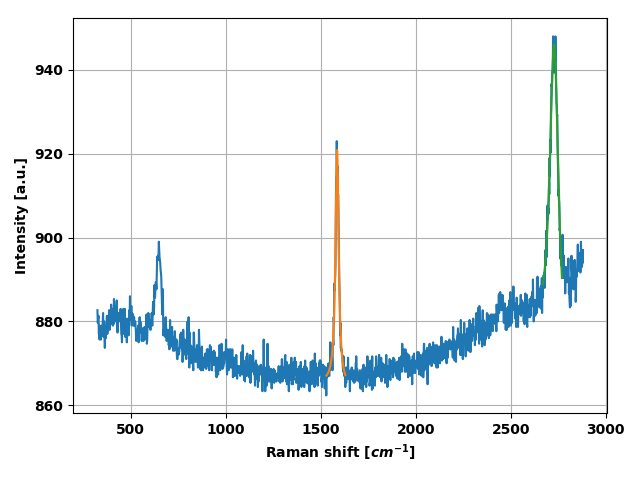
\includegraphics[scale=0.5]{Bilder/part6/6.png}
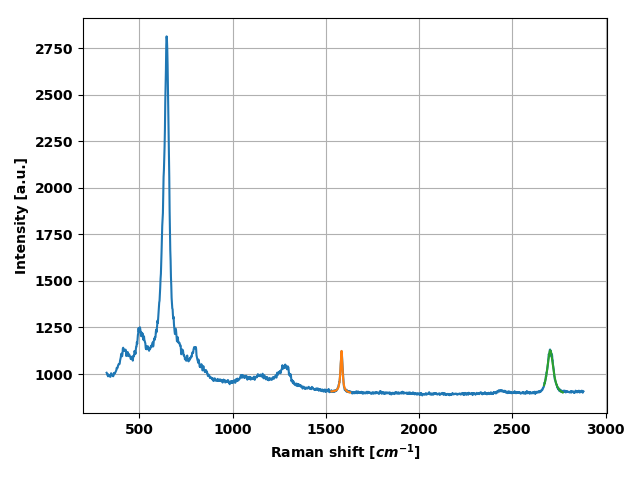
\includegraphics[scale=0.5]{Bilder/part6/7.png}
\caption{Spectra of the sample on polycristalline Cu. Top left is Measurement point 1 and bottom right point 7. The fits to the G and 2D-line are included.}
\label{fig:appendix_6}
\end{figure}

\end{document}